\documentclass[12pt,a4paper,austrian]{article}
\usepackage{graphicx}
\usepackage[austrian, english]{babel}
\usepackage[utf8]{inputenc}
\usepackage{listings}
\usepackage{multirow}
\usepackage{epstopdf}
\usepackage{amsmath}
\usepackage{amssymb} % fuer Mengen \N, Q, C, R
\graphicspath{{./fig/}}


%% Satzspiegel
\setlength{\hoffset}{-1in} \setlength{\textwidth}{18cm}
\setlength{\oddsidemargin}{1.5cm}
\setlength{\evensidemargin}{1.5cm}
\setlength{\marginparsep}{0.7em}
\setlength{\marginparwidth}{0.5cm}

\setlength{\voffset}{-1.9in}
\setlength{\headheight}{12pt}
\setlength{\topmargin}{2.6cm}
   \addtolength{\topmargin}{-\headheight}
\setlength{\headsep}{3.5cm}
   \addtolength{\headsep}{-\topmargin}
   \addtolength{\headsep}{-\headheight}
\setlength{\textheight}{27cm}

%% How should floats be treated?
\setlength{\floatsep}{12 pt plus 0 pt minus 8 pt}
\setlength{\textfloatsep}{12 pt plus 0pt minus 8 pt}
\setlength{\intextsep}{12 pt plus 0pt minus 8 pt}

\tolerance2000
\emergencystretch20pt

%% Text appearence
% English text
\newcommand{\eg}[1]%
  {\selectlanguage{english}\textit{#1}\selectlanguage{austrian}}

\newcommand{\filename}[1]
  {\begin{small}\texttt{#1}\end{small}}

\newcommand\IFT{\unitlength1mm\begin{picture}(10,2) \put (1,1)
{\circle{1.7}} \put(2,1){\line(1,0){5}} \put(8,1)
{\circle*{1.7}}\end{picture}}
\newcommand\FT{\unitlength1mm\begin{picture}(10,2) \put (1,1)
{\circle*{1.7}} \put(2,1){\line(1,0){5}} \put(8,1)
{\circle{1.7}}\end{picture}}

% A box for multiple choice problems
\newcommand{\choicebox}{\fbox{\rule{0pt}{0.5ex}\rule{0.5ex}{0pt}}}

\newenvironment{wahrfalsch}%
  {\bigskip\par\noindent\makebox[1cm][c]{richtig}\hspace{3mm}\makebox[1cm][c]{falsch}
   \begin{list}%
   {\makebox[1cm][c]{\choicebox}\hspace{3mm}\makebox[1cm][c]{\choicebox}}%
   {\setlength{\labelwidth}{2.31 cm}\setlength{\labelsep}{3mm}
    \setlength{\leftmargin}{2.61 cm}\setlength{\listparindent}{0pt}
    \setlength{\itemindent}{0pt}}%
  }
  {\end{list}}

\newcounter{theaufgabe}\setcounter{theaufgabe}{1}
\newenvironment{aufgabe}[1]%
  {\bigskip\par\noindent\begin{nopagebreak}
   \textsf{\textbf{\arabic{theaufgabe}.\thinspace Aufgabe}}\quad
      \textsf{\textit{#1}}\\*[1ex]%
\stepcounter{theaufgabe}\hspace{2ex}\end{nopagebreak}}
  {\par\pagebreak[2]}

% Innerhalb der Aufgaben erfolgt die weitere Unterteilung mittels einer
% enumerate Umgebung, die allerdings a), b),... zaehlen soll.
\renewcommand{\labelenumi}{\alph{enumi})}
\renewcommand{\labelenumii}{\arabic{enumii})}

% A box to tick for everything which has to done
\newcommand{\abgabe}{\marginpar{$\Box$}}
% Margin paragraphs on the left side
\reversemarginpar

% Language for listings
\lstset{language=Vhdl,
  basicstyle=\small\tt,
  keywordstyle=\tt\bf,
  commentstyle=\sl}

% No indention
\setlength{\parindent}{0.0cm}
% Don't number sections
\setcounter{secnumdepth}{0}


%% Beginning of the text

\begin{document}
\selectlanguage{austrian}
\pagestyle{plain}
% This is the header section
  \thispagestyle{empty}
  \noindent
  %\includegraphics[height=2.5cm]{fig/JKULogoFullEnglShort}
  % blagOPP
  \begin{minipage}[b][2.4cm]{1.0\textwidth}  
  \begin{tabular}{l p{11cm} r} 
    \multicolumn{3}{c}{\centering \begin{large}\begin{bf}
  	\textsf{Digitale Signalverarbeitung, WS 2019/20} \end{bf}\end{large} }  
  	 \\
  	\multirow{2}{*}{
\includegraphics[height=1.6cm]{fig/JKU_Logo}} 
  	& \centering Bernhard Fürst k0442418, Sebastian Ortner kxxxxxx, Gruppe 34 \vspace{1.3em}  &
    \multirow{2}{*}{
\includegraphics[height=1.9cm]{fig/ISP-Logo-color-02}}  \\	
    & \centering \textit{1. Übung} & \\     
    \multicolumn{3}{c}{\centering \begin{large}
    \textit{Überschrift der Übung}%
    \end{large} }  
 
  \end{tabular} 
  \end{minipage}
%  \vspace{-1.2em}

  \noindent \rule[0.8em]{\textwidth}{0.12mm}\\[-0.5em]

%%%%%%%%%%%%%%%%%%%%%%%%%%%%%%%%%%%%%%%%%%%%%%%%%%%%%%%%%%%%%%%%%%%%%%%%%%%%%%



\begin{aufgabe}{}
  \begin{enumerate}
    \item [a)]
  \end{enumerate}
\hspace{-2cm}
  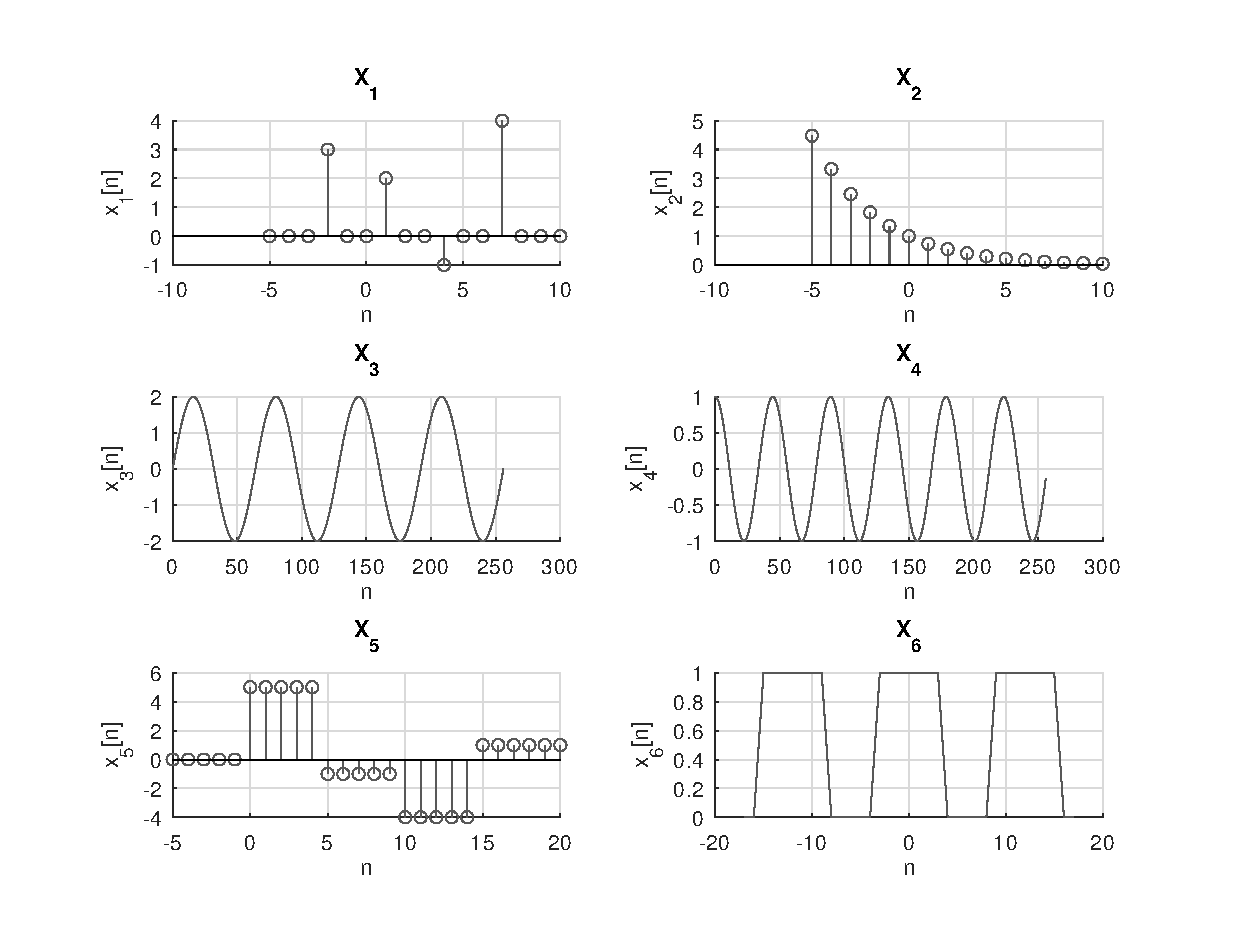
\includegraphics{x1_6.eps}
  \begin{enumerate}
      \item [b)]
      \begin{itemize}
        \item $x_3 \rightarrow f_0 = \frac{\frac{2\pi}{64}}{1} \Rightarrow  \Omega_0 = \frac{2\pi}{64}$
        \item $x_4 \rightarrow f_0 = \frac{9}{64*2\pi} \Rightarrow \frac{9}{64}$
      \end{itemize}
      \item [c)]
      \begin{itemize}
        \item $x_3$ ist periodisch, die Periodendauer ist abzulesen bei x= 64.
        \item $x_4 \rightarrow n = \frac{2\pi k}{\frac{9}{64}}\Rightarrow \frac{2\pi * 64 k}{9}$ \\k müsste eine irrationale Zahl sein damit n ein Element aus den ganzen Zahlen ist. Zu diesem diskreten Punkt gibt es keine Periodendauer. 
      \end{itemize}
      \item [d)]
  \end{enumerate}
\end{aufgabe}
\begin{aufgabe}{}
 a 
\end{aufgabe}
\begin{aufgabe}{}
  Der Durchschnitt unserer Dreiecksfunktion ist $0$ was leicht anhand der Symmetrie bezüglich der x-Achse gesehen werden kann. Damit ist auch der DC-Anteil der Fourierreihe, $a_0$, $0$.
    Dies kann auch folgendermassen gezeigt werden :
    
    \begin{eqnarray*}
        a_{0} &=\frac{1}{T}\int_{0}^{T}f(t)dt 
    \end{eqnarray*}

Aufgrund der Symmetrie in der Funktion erkennen wir dass das Integral von $0$ nach $\frac{T_0}{2}$ gleich dem Integral von $\frac{T_0}{2}$ nach $T_0$ sein muss. Daher können wir sagen dass :
\begin{equation}
    a_0=\frac{2}{T_0}\int_{0}^{\frac{T_0}{2}}f(t)dt 
\end{equation}

Wir können uns nun auf einen Teil der zweiteiligen Funktion beschränken. Da die Funktion an der Strecke von $0$ nach $\frac{T}{2}$ die Form $A-\frac{4A}{T}$ hat gilt :
\begin{eqnarray*}
    a_0=&\frac{2}{T_0}\int_{0}^{\frac{T_0}{2}}A-\frac{4A}{T_0}tdt \\
    =&\frac{2}{T_0}(At-\frac{4A}{T_0}\frac{t^2}{2})\big |_0^{\frac{T_0}{2}}\\
    =&\frac{2}{T_0}(A\frac{T_0}{2}-\frac{2A\frac{T_0^2}{4}}{T_0}-A0-\frac{2A\frac{0}{4}}{T_0})\\
    =&\frac{2}{T_0}(A\frac{T_0}{2}-\frac{AT_0^2}{2T_0}-0-0)\\
    =&\frac{2}{T_0}(A\frac{T_0}{2}-A\frac{T_0}{2}-0) \\ =& \underline{0}
\end{eqnarray*}

\pagebreak

    Um $a_n$ zu finden können wir, wieder aufgrund der oben festgestellten Symmetrie, folgenden Term evaluieren :
    \begin{eqnarray*}
        a_n = & \frac{4}{T}\int_{0}^{\frac{T}{2}}f(t)\cos\omega ntdt\\
        =&\frac{4}{T}\int_{0}^{\frac{T}{2}}(A-\frac{4A}{T}t)\cos\omega ntdt \\
        =&\frac{A4}{T}\int_{0}^{\frac{T}{2}}(1-\frac{4}{T}t)\cos\omega ntdt \\
        =&\frac{A4}{T}(\int_{0}^{\frac{T}{2}}\cos\omega ntdt-\int_{0}^{\frac{T}{2}}\frac{4}{T}t\cos\omega ntdt)\\
        =&\frac{A4}{T}((\frac{1}{\omega n}\sin\omega nt)\big |_0^{T}-\int_{0}^{\frac{T}{2}}\frac{4}{T}t\cos\omega ntdt)\\
        =&\frac{A4}{T}((\frac{1}{\omega n}\sin\frac{2\pi}{T} n\frac{T}{2}-(\frac{1}{\omega nt}\sin\frac{2\pi}{T} n 0)-\int_{0}^{\frac{T}{2}}\frac{4}{T}t\cos\omega ntdt)\\
        =&\frac{A4}{T}((\frac{1}{\omega n}\sin \pi n- 0 -\int_{0}^{\frac{T}{2}}\frac{4}{T}t\cos\omega ntdt)
    \end{eqnarray*}
    Ganzzahlige Vielfache von pi ergeben immer einen Sinus von 0.
    \begin{eqnarray*}
        a_n = & \frac{A4}{T}(0 - 0 -\int_{0}^{\frac{T}{2}}\frac{4}{T}t\cos\omega ntdt)\\
         = & \frac{A4}{T}\int_{0}^{\frac{T}{2}}\frac{-4}{T}t\cos\omega ntdt\\
         = & \frac{-16A}{T^2}\int_{0}^{\frac{T}{2}}t\cos\omega ntdt\\
         = & \frac{-16A}{T^2}((t \frac{1}{\omega n}\sin \omega n t)\big |_0^\frac{T}{2}-\int_0^{\frac{T}{2}}\frac{1}{\omega n}\sin \omega ntdt)\\
         = & \frac{-16A}{T^2}(( \frac{\frac{T}{2}}{\omega n}\sin \frac{2\pi}{T} n \frac{T}{2} - \frac{1}{\omega n}\sin 0) -\int_0^{\frac{T}{2}}\frac{1}{\omega n}\sin \omega ntdt)\\
         = & \frac{-16A}{T^2}(( \frac{\frac{T}{2}}{\omega n}\sin \pi n -  0) -\int_0^{\frac{T}{2}}\frac{1}{\omega n}\sin \omega ntdt)\\
         = & \frac{-16A}{T^2}( 0 -\int_0^{\frac{T}{2}}\frac{1}{\omega n}\sin \omega ntdt)\\
         = & \frac{16A}{T^2}(\frac{-1}{\omega^2 n^2}\cos\omega n t )\big |_0^{\frac{T}{2}}\\
         = & \frac{16A}{T^2}\frac{1}{\omega^2 n^2}(-\cos\omega n t )\big |_0^{\frac{T}{2}}\\
         = & \frac{4A}{\pi^2 n^2}(-\cos\frac{2\pi}{T}n\frac{T}{2}+\cos 0)\\
         = & \frac{4A}{\pi^2 n^2}(-\cos\pi n + 1)
    \end{eqnarray*}

    Bei ungeraden Werten von n evaluiert dieser Term zu $\frac{8A}{\pi^2 n^2}$ bei geraden zu $0$ da der Cosinus bei ungeraden Vielfachen von $\pi -1$ annimmt und bei geraden 1. 


    Der Faktor $b_n$ ist bei geraden periodischen Funktionen, d.h. periodischen Funktionen die symmetrisch zur y-Achse sind, immer 0.
    
    Eingesetzt in die Fourierreihe erhalten wir nun.

    \begin{eqnarray*}
        x(t) = &  \sum_{n=1}^\infty \frac{8A}{\pi^2 (2n-1)^2}\cos(2\pi (2n-1) f_0 t)
        =& \frac{8A}{\pi^2}\sum_{n=1}^\infty\frac{\cos(2\pi (2n-1) f_0 t)}{(2n-1)^2}
    \end{eqnarray*}

    $n$ schreitet voran als $2n-1$ da wir nur an ungeraden Werten interessiert sind.
\end{aufgabe}

\end{document}
